\begin{figure}[!ht]
\centering
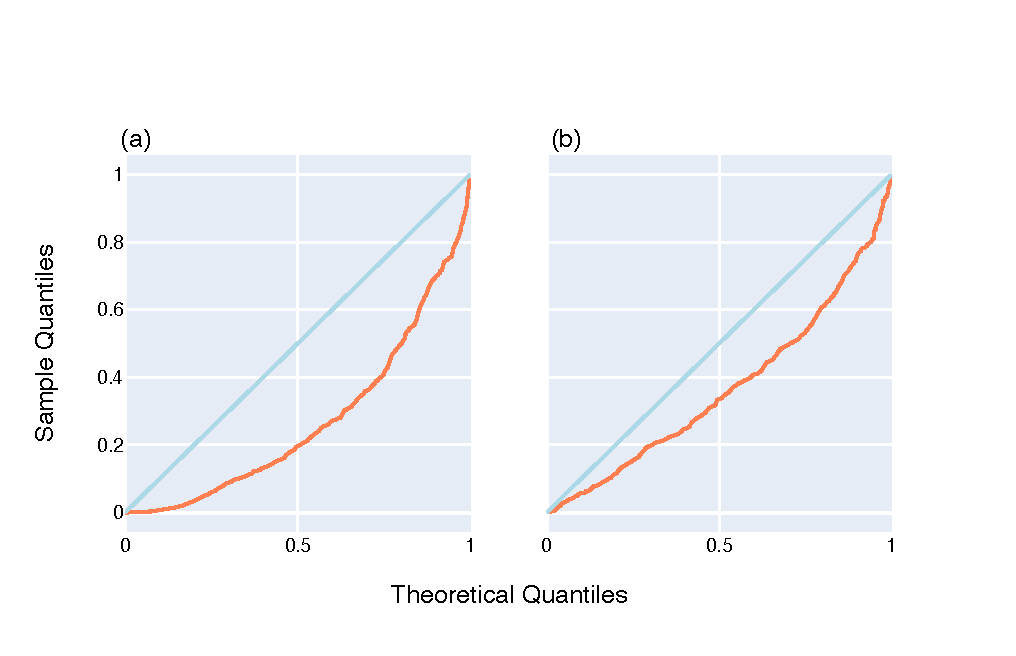
\includegraphics[width=\textwidth]{figures/plots/synthetic/lrt/197113_332182_17210-long_seq.pdf}
\caption{\textbf{Increasing the length of the alignments gives a distribution of $\hat p-$ values closer, but not consistent with theoretical expectations.} The Quantile-Quantile (Q-Q) plots compare the $\hat p$-value distribution of the test for existence in stationary simulated data to the uniform distribution. If the distributions were identical, the data points (shown as the red line) would fall on the diagonal (indicated by the blue line). \textbf{(a)} Q-Q plot for synthetic alignments of length $300$, for which the data points fall well below the diagonal. \textbf{(b)} Q-Q plot for synthetic alignments of length $30,000$. Owing to increasing the power of the test, the data points fall much closer to the diagonal line. Although closer for longer sequences, both data sets are not consistent the theoretical expectations. This result indicates that the test for existence yields an excess of small $p-$ values, and for all lengths requires bootstraps to robustly estimate significance. Both data sets shown are generated from the same high JSD, high entropy seed. The other seeds exhibited the same pattern, the result is shown in the appendix Figure \ref{fig:synthetic/lrt/all-seeds}.}
\label{fig:synthetic/lrt/197113-long_seq}
\end{figure}